%%%%%%%%%%%%%%%%%%%%%%%%%%%%%%%%%%%%%%%%%%%%%%%%%%%%%%%%%%%%%%%%%%%%
\section{Handling and Transport to SURF} % and Receiving at the DUNE Integration Facility}
\label{sec:fdsp-apa-transport}

Completed \dword{apa}s are shipped from the \dword{apa} production sites to 
the \dword{sdwf} in South Dakota. As they are transported to the \dword{4850l}, they are integrated %  for integration 
with the \dword{tpc} \dword{fe} electronics and \dwords{pd} followed by installation in the cryostat. %\dword{dune} cryostats.  %The \dword{itf} location is not yet confirmed, but facilities near the \surf site are being considered.   
Extensive \dword{qc} testing will be performed before installation to ensure the fully integrated \dword{apa}s function properly.  %Once checked, the \dword{apa}s are repackaged for final transport to \surf.  
Installation activities at \dword{surf} are described in Chapter~\ref{ch:sp-install}. 

%%%%%%%%%%%%%%%%%%%%%%%%%%%%%%%%%%%%%%%%%%%%%%%%%%%%%%%%%%%%%%%%%%%%
\subsection{APA Handling}
\label{sec:fdsp-apa-transport-handling}

The handling of the \dword{apa}s  must %throughout their lifetime must be carefully considered to 
ensure their safety.  Several lifting and handling fixtures will be employed for transferring and manipulating the \dword{apa}s during fabrication, integration, and installation.  At the production sites a fixture called the edge lift kit will be used to transfer the \dword{apa} to and from the process cart and the winder, as well as to the transport containers.  The lift kit is shown schematically in Figure~\ref{fig:apa-edge-lift}.  It is essential that the fixture connect to the \dword{apa} along an outer edge because after wires are attached to the support frame, it can no longer be grabbed anywhere on the front or back face of the frame. 
%The edge lift kit will also be used to transfer the \dword{apa} from the transport frame to a process cart there.  

\begin{dunefigure}[APA edge lifting fixture]{fig:apa-edge-lift}
{A custom lifting fixture is used to pick up an \dword{apa} from the long edge and safely handle it during the various construction steps at the production sites.}  
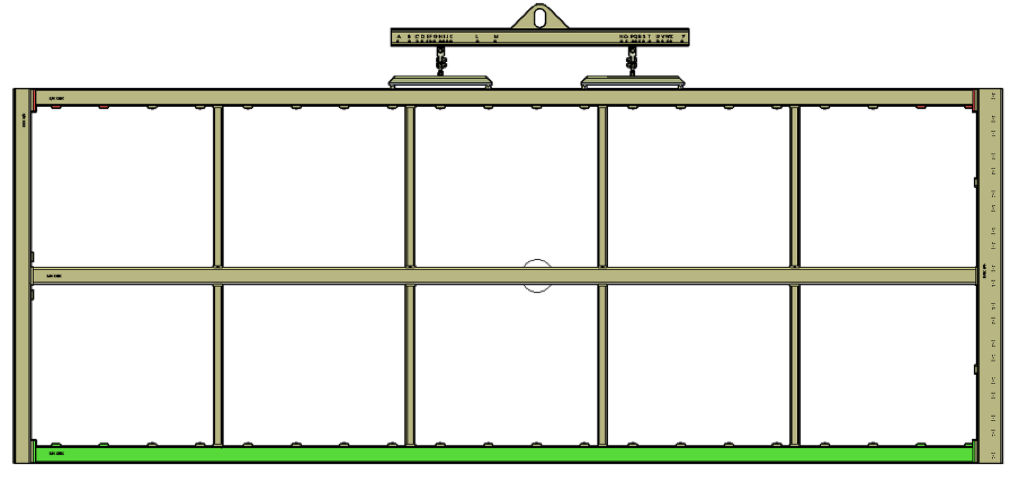
\includegraphics[width=0.8\textwidth]{sp-apa-edge-lift-kit.png} 
\end{dunefigure}

%%%%%%%%%%%%%%%%%%%%%%%%%%%%%%%%%%%%%%%%%%%%%%%%%%%%%%%%%%%%%%%
\subsection{APA Transport Frame and Shipping Strategy}
\label{sec:fdsp-apa-transport-container}


The transport packaging for the \dword{apa}s is designed to safely transport them from the production sites to the \dword{sdwf}. %underground clean room in the detector hall at \dword{surf}. 
The design of the packaging is shown in Figure~\ref{fig:apa-transport-frame}. Light rigid metalized foam protective panels are attached via clamps affixed to the \dword{apa} frames and provide the primary protection for the wire planes. Pairs of \dword{apa}s (one upper and one lower in an \dword{apa} pair) are loaded onto welded structural steel transport frames at the factory. The \dword{apa} frames are bolted to mounts on the transport frames that incorporate shock-attenuating coil springs designed to reduce possible accelerations on the \dword{apa} frames to less than $4g$. The \dword{apa}s and transport frames will be instrumented with accelerometers to %understand 
find out if the \dword{apa}s were subject to shocks above their specifications. Removable side frames, made from aluminum, are then bolted to the transport frames providing a structure around the \dword{apa}s, and this whole structure is then %wrapped in 
sealed in plastic sheeting. 

The packaged transport frames from the US sites will be covered in wooden panels, loaded on custom pallets, and shipped via truck from the \dword{apa} factories to the \dword{sdwf}. %) near Rapid City. 
The packaged transport frames from the UK will be packed, in pairs, inside wooden crates for shipping. They then will be trucked to the nearby port in Liverpool, transported by ship to the port of Baltimore, and then shipped by truck to the \dword{sdwf}. %In some cases, t
\dword{apa}s may be stored for three years or longer at the \dword{sdwf} -- an \dword{apa} crate cannot arrive at \dword{surf} until it is required underground. 

\begin{dunefigure}[APA transport frame]{fig:apa-transport-frame}
{The current design of the APA shipping frame (maroon) and removable side frames (green) with two APAs covered with protective panels (shown in grey and tan). The external wooden packaging is not shown in this view.}  
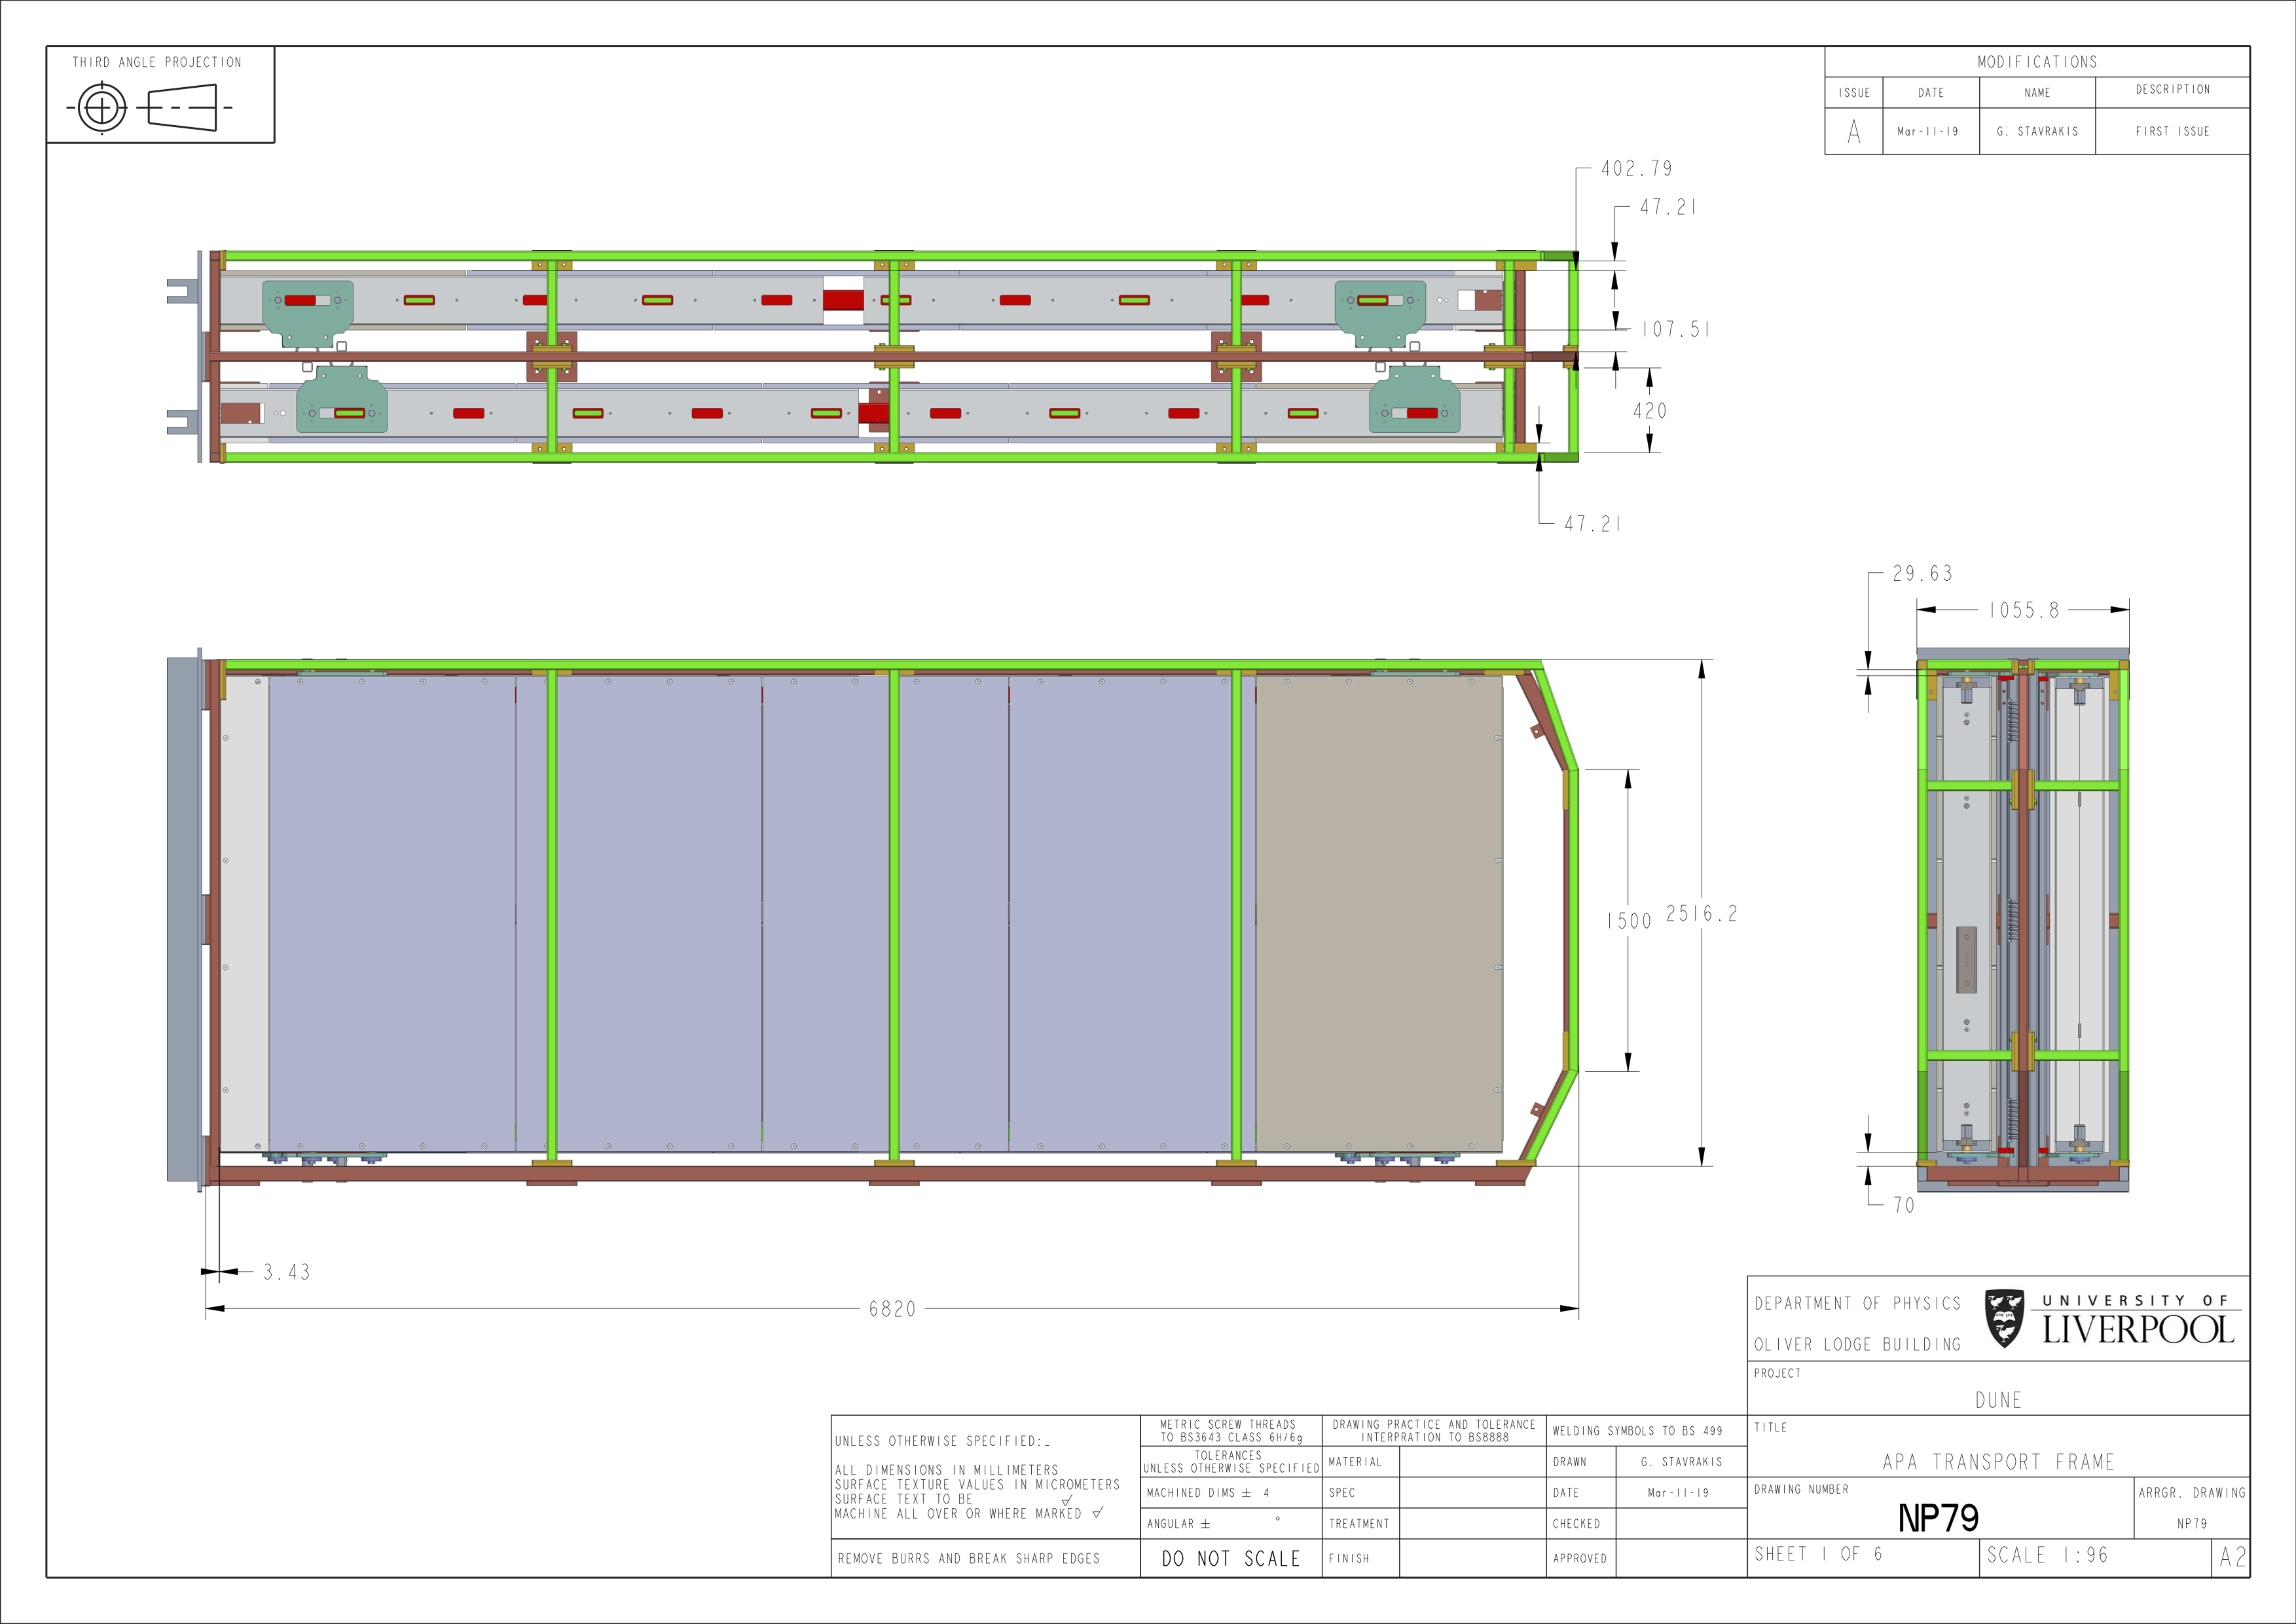
\includegraphics[width=0.9\textwidth]{graphics/sp-apa-transport-box-drawing.png} 
\end{dunefigure}
% No more ITF - changed to SDWF

The size of the packaging and rigging hardware is constrained by the Ross headframe dimensions and over-the-road shipping requirements in the US. The design of the protective panels and the side frames allow for temporarily removing a portion of the shipping packaging and protective panels to access the \dword{apa} head boards for wire tension, isolation, and continuity tests after shipment and after transport underground. 

When a crate is required underground, %the crates 
it will be stripped of its wooden crating and %then
 transported via Conestoga-type trailer to the headframe area. Near the headframe, the crates will be moved by forklift onto a cart on a rail system and rolled into the headframe. The inside portion of the headframe will have rigging gear attached to hard points on both short ends of the crate. %One end (upper end) 
 The crate's upper end will be attached %used for attaching 
 to the hoist below the cage and will be used to lift the crate from horizontal to vertical and pull it into the shaft. The shipping frame is designed to clear the headframe during this operation. The other end (lower) will be used to attach a horizontal tugger that will control the crate as it is pulled into the shaft station (Figure~\ref{fig:apa-transport-shaft}). When in the shaft, fixtures on the sides of the crate will engage wooden guides in the shaft to keep the crate from swinging or rotating while being lowered down the shaft. This operation is consistent with standard slung-load transport procedures at \dword{surf}. When the crate arrives underground, it will be pulled out of the shaft by reversing the shaft rigging operation; it will land on the opposite long edge of the crate that was used on the surface. The crate is placed on a transport cart and pulled down the drift to the cavern. When in the cavern, the \dword{apa}s will be uncrated, rotated to vertical by the cavern crane, mounted on a vertically oriented cart, tested, and stored temporarily (a few weeks) in the cavern adjacent to the clean room prior to final integration and installation. The transport frames and carts have been designed to be stable in each of these configurations. 

\begin{dunefigure}[APA loading into the mine shaft]{fig:apa-transport-shaft}
{Motion study of loading an \dword{apa} frame into the shaft.}  
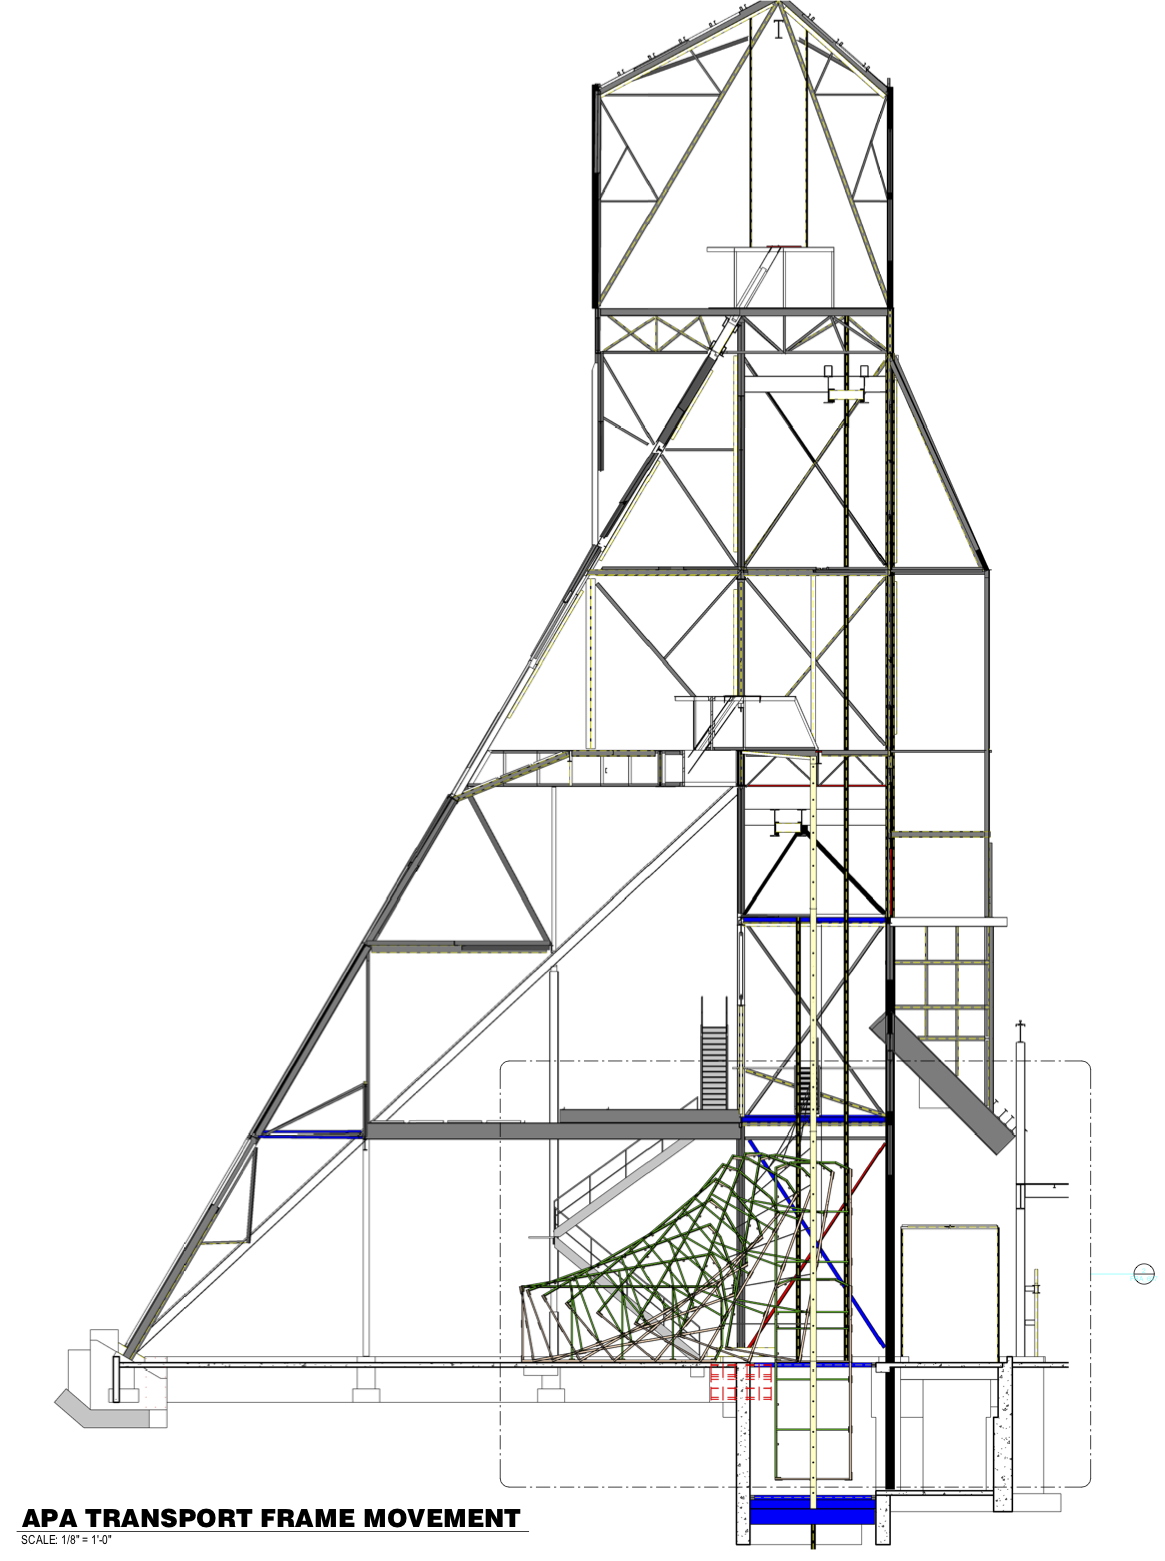
\includegraphics[height=0.9\textheight,trim = 0mm 0mm 0mm 0mm, clip]{graphics/sp-apa-transport-shaft.png} 
\end{dunefigure}

%%%%%%%%%%%%%%%%%%%%%%%%%%%%%%%%%%%%%%%%%%%%%%%%%%%%%%%%%%%%%%%%%%%%
\subsection{APA Quality Control During Integration and Installation} 
\label{sec:fdsp-apa-transport-qc}

All active detector components are shipped to the \dword{sdwf} before final transport to \dword{surf}. 
After unpacking an \dword{apa} (underground at \dword{surf}), a visual inspection will be performed and wire continuity and tension measurements will be made. 
Tension values will be recorded in the database and compared with the original tension measurements performed at the production sites, as was done for \dword{pdsp} and shown in Figure~\ref{fig:sp-apa-pd-tension-cern}. Definite guidance for the acceptable tension values will be available to inform decisions on the quality of the \dword{apa}. Clear pass/fail criteria % I think slash ok in this construction; leaving it in (anne)
will be provided as well as clear procedures to deal with individual wires lying outside the acceptable values. %Exact relation between lower or higher tension and the acceptance of a channel still needs to be worked out. 
This guidance will be informed also by the \dword{pdsp} experience. %, where the tension of some wires changed during the production to installation process. 
In addition, a continuity test and a leakage current test is performed on all channels and the data recorded in the database. 


When all tests are successful, 
the \dword{apa} can be prepared 
for integration with the other components. % Integration and final testing will take place underground. %; there we will have more time available to perform tests. 
This step is critical for ensuring high performance of the integrated \dword{apa}s. The procedures for \dword{apa} transport to the \dword{4850l} at \dword{surf}, integration with the \dword{pds} and \dword{ce}, and the schedule for testing the integrated \dword{apa} are addressed in %the Technical Coordination Chapter of the \dword{dune} TDR.
Chapter~\ref{ch:sp-install}. \dword{apa} consortium personnel will play direct and key roles throughout the integration and installation activities.  



